\documentclass[a4paper]{article}
\usepackage{subfig}
\usepackage[pdftex]{graphicx}
\graphicspath{{../figures/}}
\DeclareGraphicsExtensions{.pdf,.png}

\usepackage{hyperref}
\usepackage{amsmath}
\usepackage{amsfonts}

\begin{document}
\title{Simulation results to Momo: Monocular Motion Estimation on Manifolds}
% author names and affiliations
% use a multiple column layout for up to three different
% affiliations
\author{Johannes Graeter\\
Institute of  Measurement and Control (MRT)\\
Karlsruhe Institute of Technology (KIT)\\
Email: johannes.graeter@kit.edu
}

% make the title area
\maketitle
\section{Remarks}
This is additional material for the paper 'Momo: Monocular Motion Estimation on Manifolds' .
Herein the simulation affected to choose the best error metric is presented in more detail.

\section{Simulation}
In order to choose the most suitable cost function and validate our algorithm, a Manhattan world is simulated and sparse optical flow is sampled on the surface of each scene element, as shown in fig.~\ref{fig:flow_simulation}.

\begin{figure}[htb]
\centering
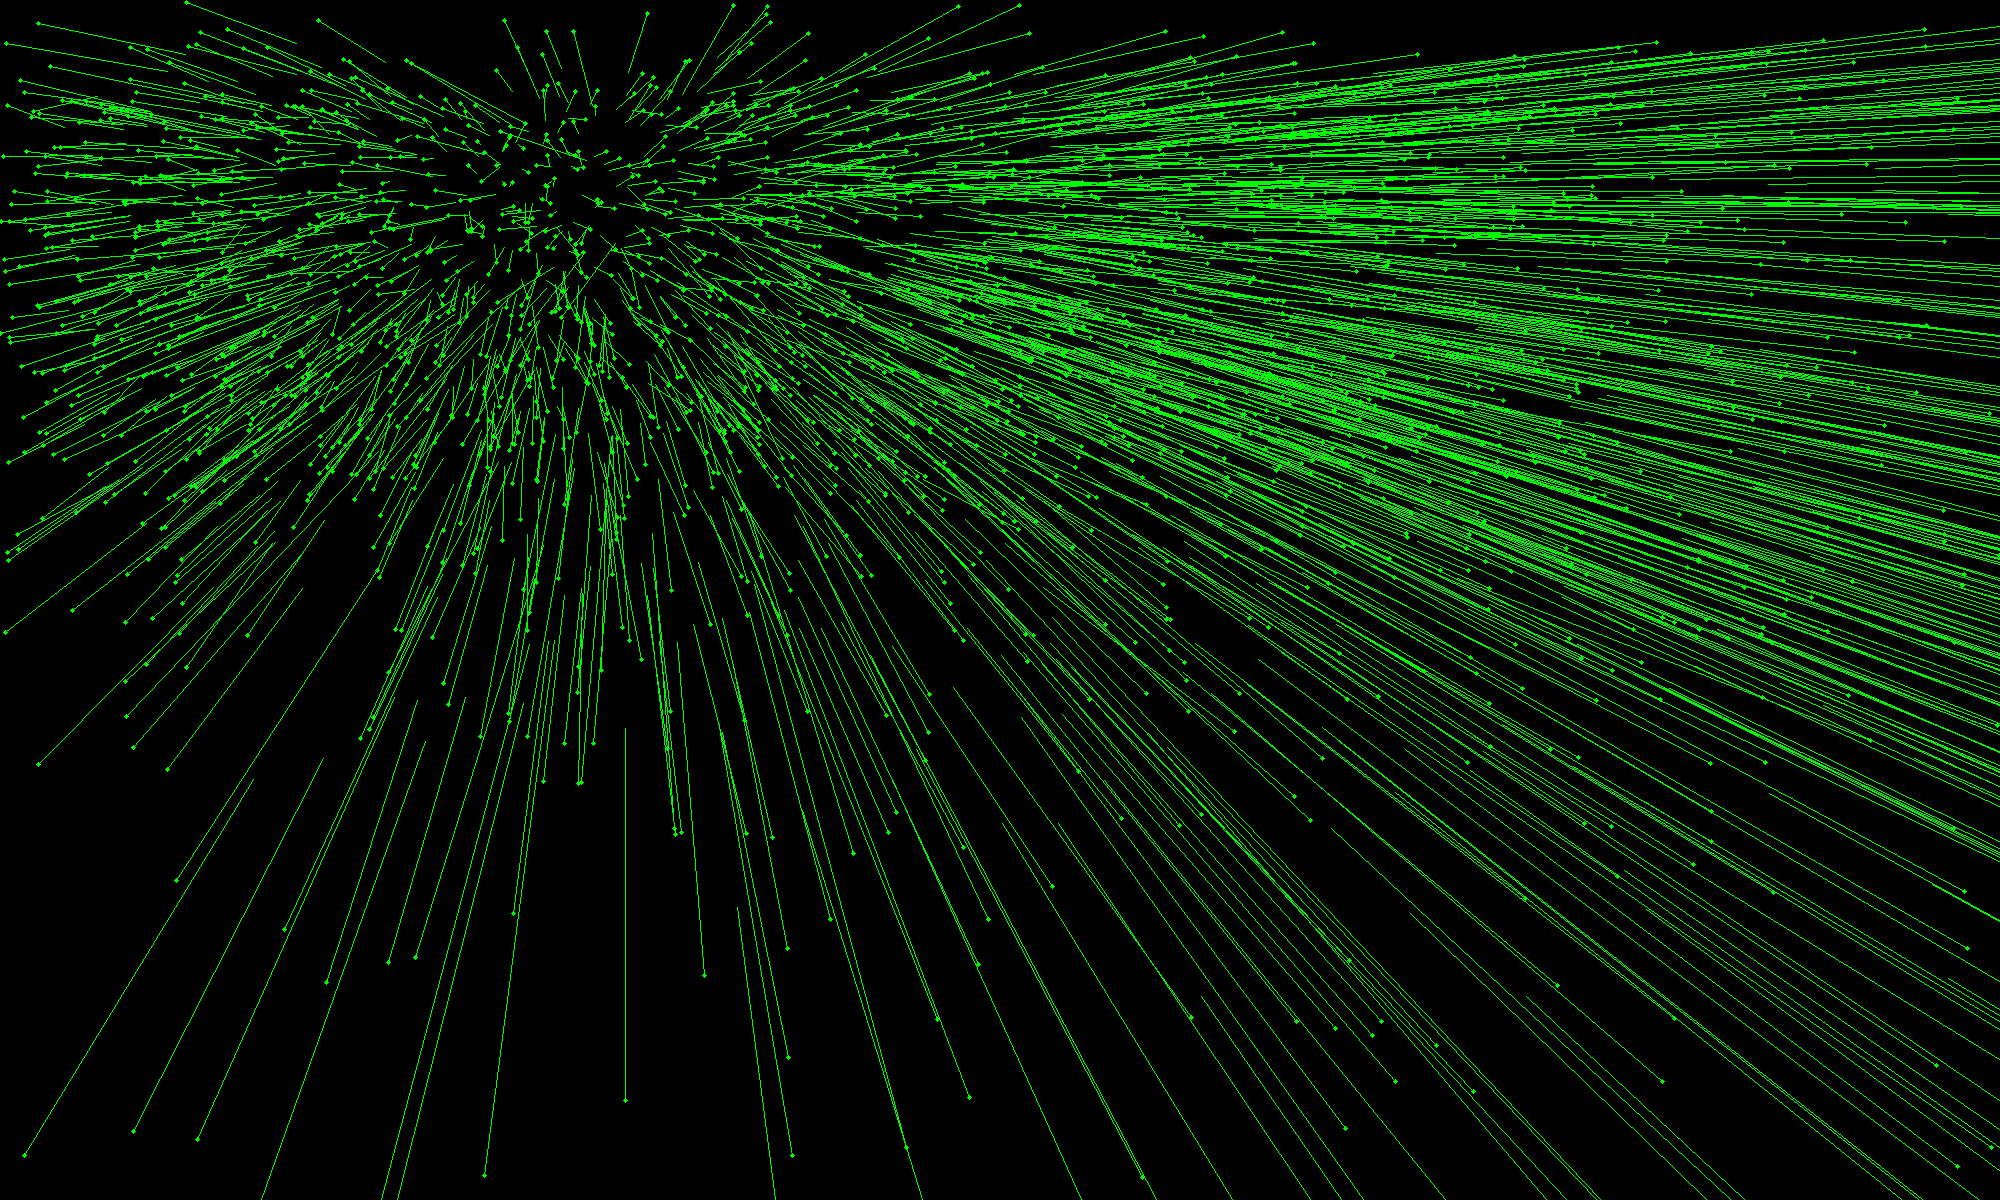
\includegraphics[width=0.8\textwidth]{flow_simulation}
\caption{Simulated flow for a vehicle movement with $\gamma=2°$ and $l=2m$. Gaussian noise is added with $standard deviation=5px$.}
\label{fig:flow_simulation}
\end{figure}

By adding gaussian noise on the simulated measurements in the image the stability of the different error functions is analysed.
Therefore the simulated flow serves as input for all three error metrics depicted in the paper.
Sampling over the dimensions of the motion state results in the error landscapes shown in fig.~\ref{fig:error_landscapes}.

\begin{figure}[htb]
\centering
\includegraphics[width=0.8\textwidth]{landscape_scale}
\caption{Error landscape for flow simulation shown in fig.~\ref{fig:flow_simulation} but without noise. We simulate one single camera, mounted as in the KITTI dataset. The red cross denotes the global minimum. The scale is correctly observed at $arc length=1.8$ }
\label{fig:landscape_scale}
\end{figure}

\begin{figure}[htb]
\centering

\subfloat[GeoLine]{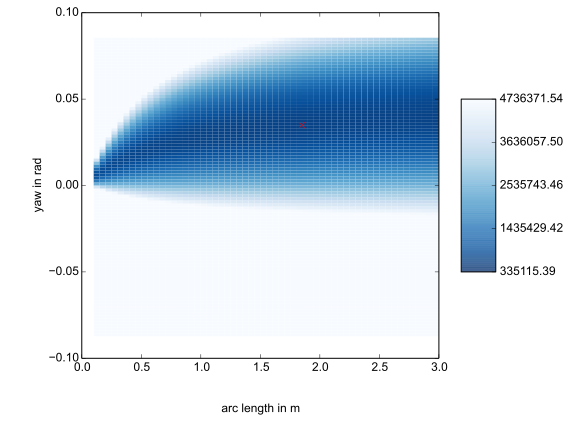
\includegraphics[width=0.8\textwidth]{cost_map_cost_epipolar_forward}%
\label{fig:error_landscapes:epipolar_forward}}
\hfil
\subfloat[AnglePlane]{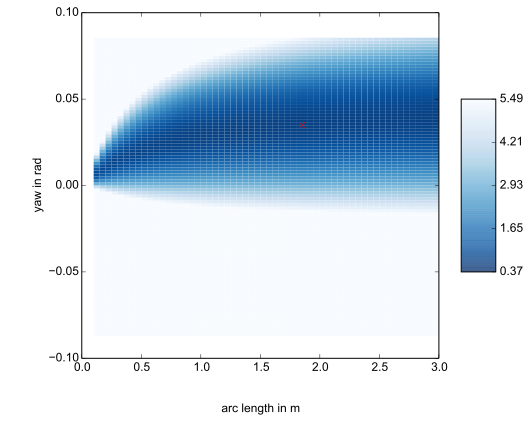
\includegraphics[width=0.8\textwidth]{cost_map_cost_geometric_linear}%
\label{fig:error_landscapes:geometric_linear}}
\hfil
\subfloat[SampLine]{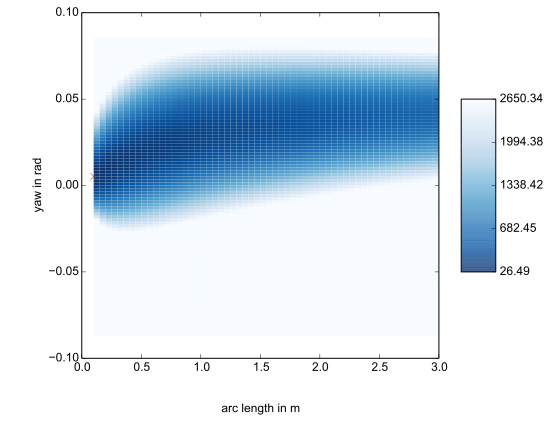
\includegraphics[width=0.8\textwidth]{cost_map_cost_sampson}%
\label{fig:error_landscapes:sampson_distance}}

\caption{Error landscapes for simulated flow as shown in fig.~\ref{fig:flow_simulation} for arc length and yaw angle of the single-track-motion-model. Whereas the shape of the landscapes of $GeoLine$ and $AnglePlane$ are nearly identical, $SampLine$ shows a valley small arc lengths, because the linearisation assumptions are violated.}
\label{fig:error_landscapes}
\end{figure}

Moreover, stability has been examined. Random noise and deviation are added to the motion estimate prior.
After 4 iterations, the error to the groundtruth is evaluated and the results are shown in the histograms in fig.~\ref{fig:histograms}.

\begin{figure}[htb]
\centering
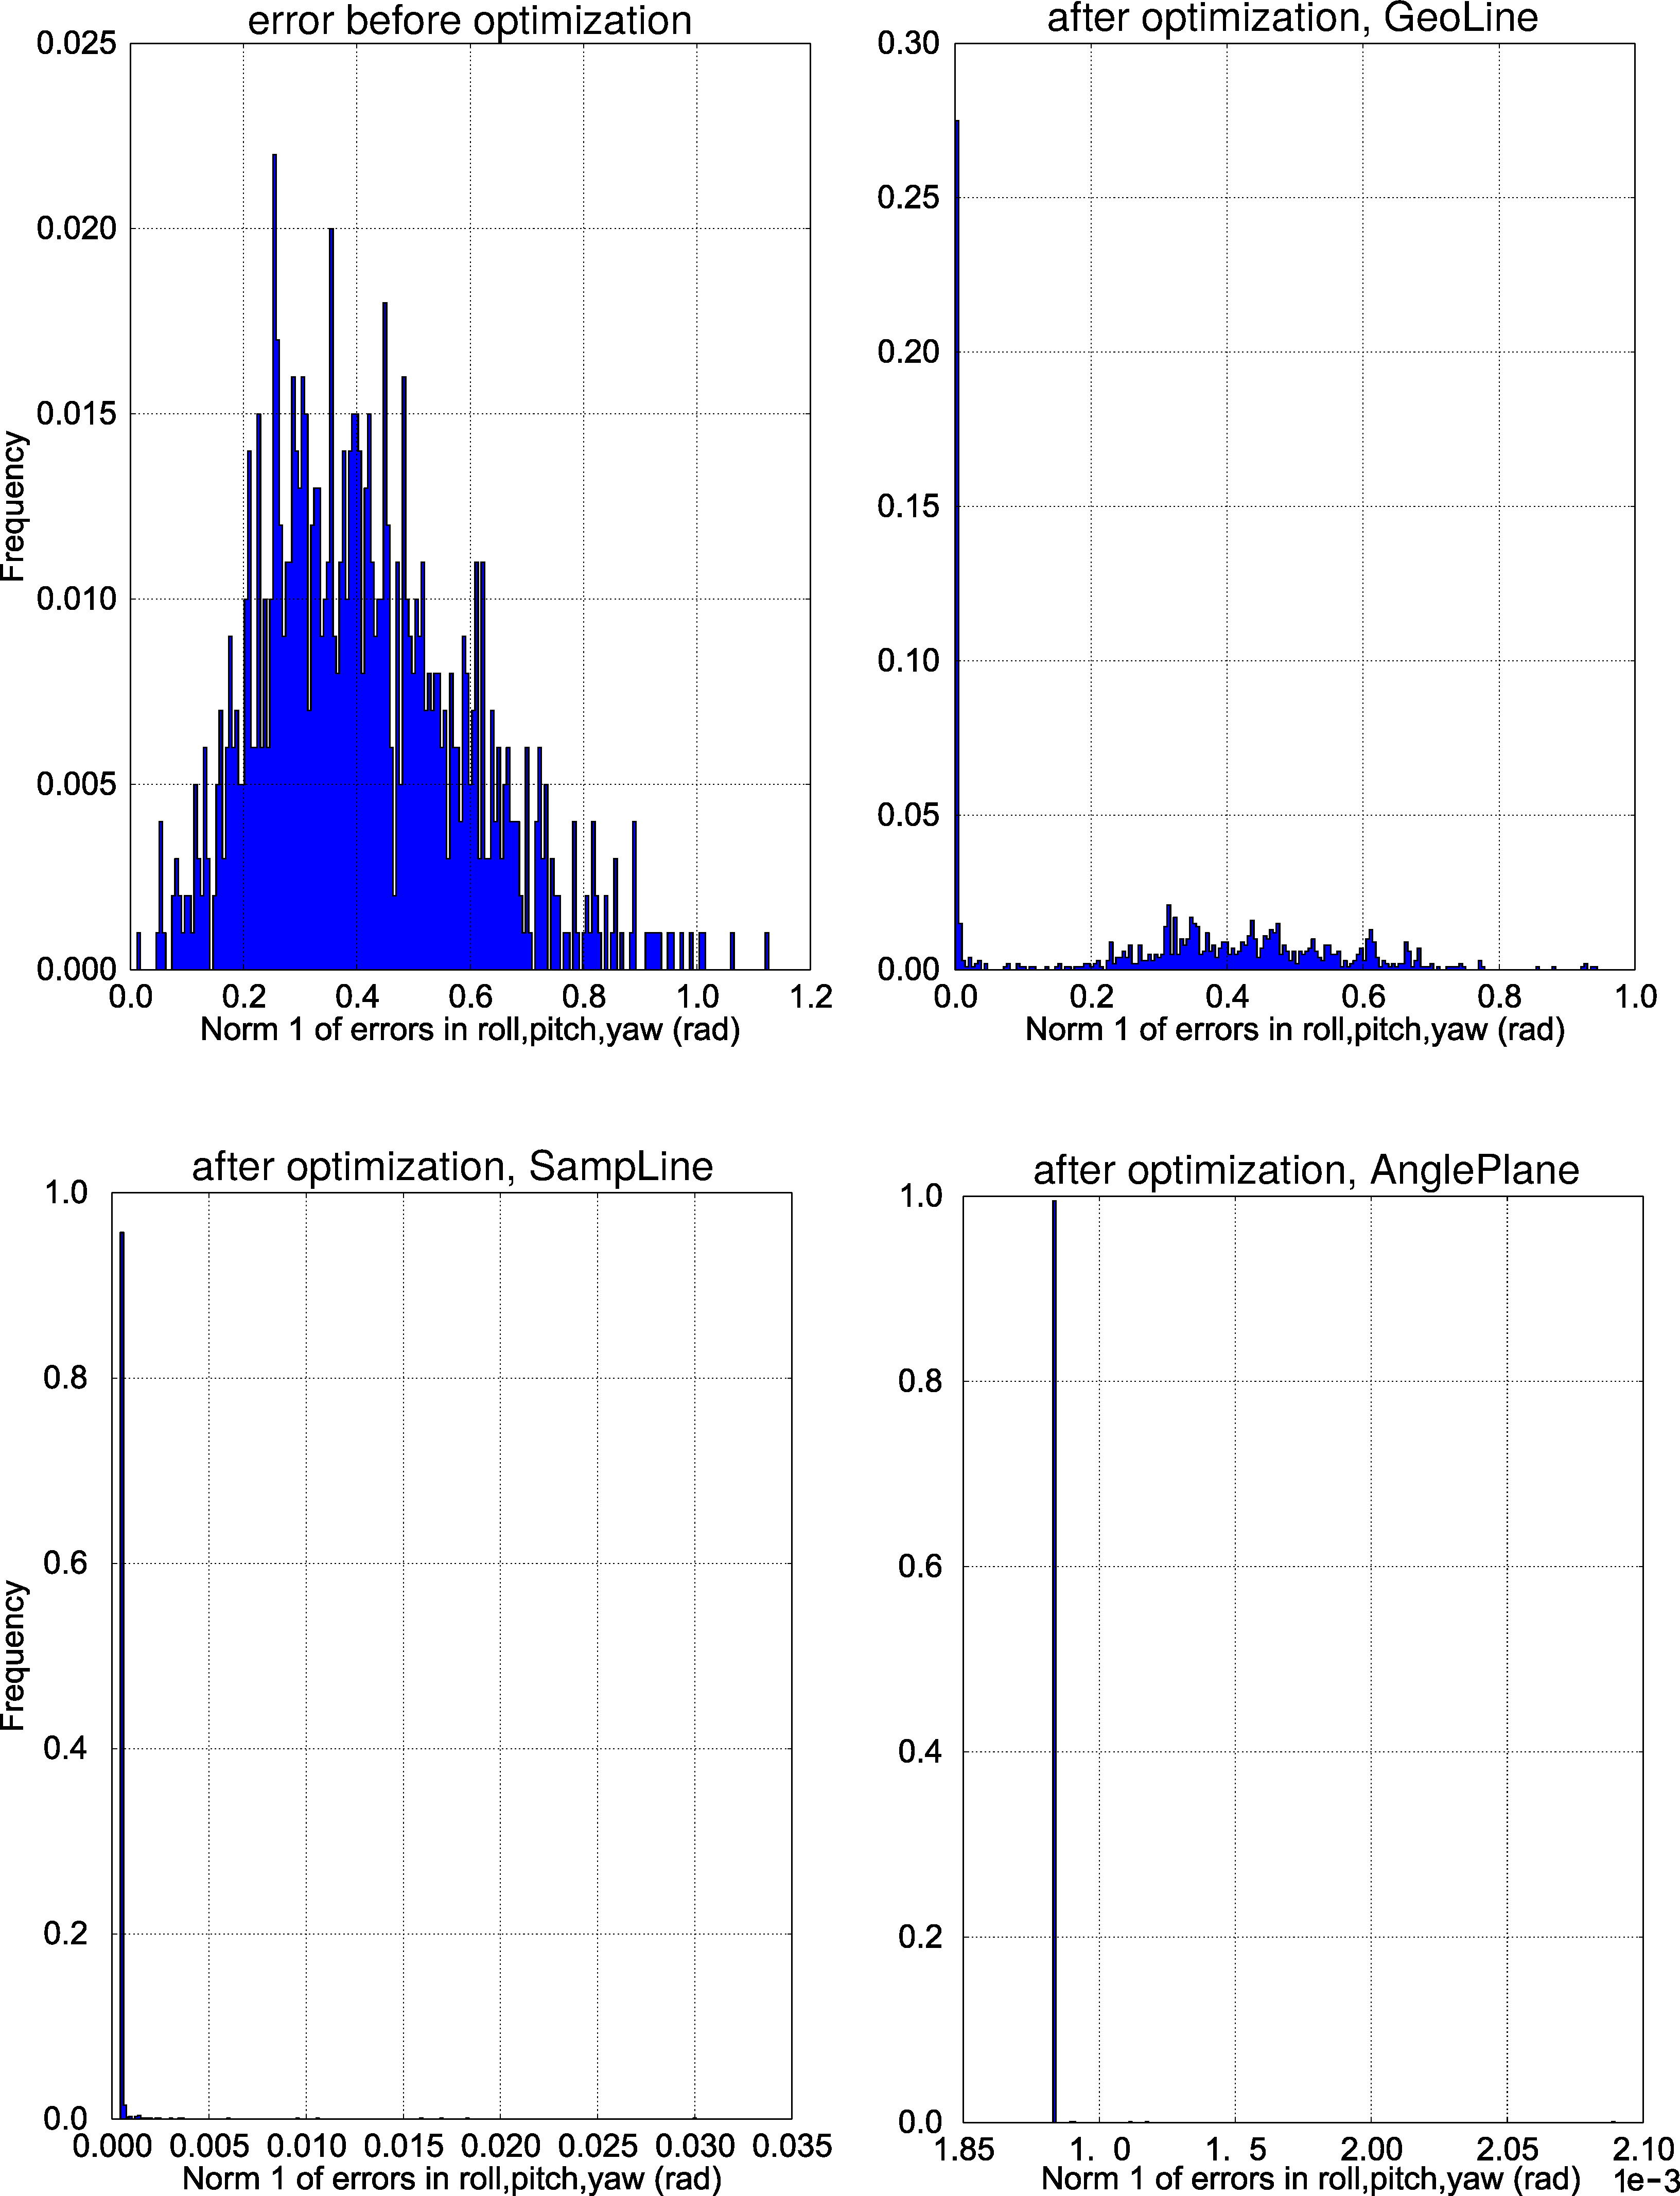
\includegraphics[width=\textwidth]{histograms_all}%
\caption{Error to groundtruth after 4 iterations. Note that $AnglePlane$ has the fastest convergence followed by $SampLine$ and $GeoLine$.}
\label{fig:histograms}
\end{figure}

As a result, both error metrics, $GeoLine$ and $AnglePlane$, are suitable choices for the potential function.
In order to enable general camera models and obtain fast convergence, $AnglePlane$ is chosen.
When an extrinsic calibration is added to the problem, the error landscape of $AnglePlane$ changes form as shown in fig.~\ref{fig:landscape_scale}.
As described in the paper the minimum of the error landscape becomes unique and the scale therefore observable. 

\end{document}